\subsubsection{\textit{Bubblesort}}

\paragraph{Lema \ref{lemma:bscount}: \texttt{bubblesort\_counts\_n2}:}
\begin{equation*}
    \forall_{l} bubblesort\_count(l)_2 = \frac{|l|^2 - |l|}{2}
\end{equation*}

\paragraph{Estratégia da prova:} direta, a partir da aplicação do
lema \ref{lemma:bacount}. O objetivo da função \texttt{bubblesort\_count}
é encapsular \texttt{bubblesort\_aux\_count}, garantindo que esta
seja chamada com os parâmetros corretos. A prova deste lema consiste
na expansão da definição de \texttt{bubblesort\_count} após instanciar
$l$ para uma lista qualquer. Nos deparamos então com os dois casos
presentes na definição de \texttt{bubblesort\_count}: o primeiro caso,
em que a lista é vazia, é trivial, pois $\frac{|l|^2 - |l|}{2} = 0$.
No segundo caso, podemos evocar o lema \ref{lemma:bacount} e instanciá-lo
adequadamente pois sabemos exatamente os valores de $c$ e $n$ que serão
passados para \texttt{bubblesort\_aux\_count}, e como eles se
relacionam com $|l|$. O comando \texttt{(grind)} utilizado nos ramos
desta prova foram utilizados para realizar as expansões da definição de
\texttt{length} e fazer as simplificações algébricas apropriadas
(Figura \ref{fig:bsort1}).

\paragraph{Lema \ref{lemma:bsequv}: \texttt{bubblesort\_equiv}:}
\begin{equation*}
    \forall_{l} bubblesort(l)_1 = bubblesort\_count(l)_1 = \frac{|l|^2 - |l|}{2}
\end{equation*}

\paragraph{Estratégia da prova:} direta, a partir da aplicação do
lema \ref{lemma:baequiv}. De forma semelhante ao lema anterior, 
a prova foi feita a partir da aplicação do lema \ref{lemma:baequiv}.
A expansão das definições de ambas \texttt{bubblesort} e \texttt{bubblesort\_count}
revela a chamada das funções \texttt{bubblesort\_aux} e \texttt{bubblesort\_aux\_count}
e a igualdade é estabelecida por meio da instanciação do lema.
Novamente, o comando \texttt{(grind)} foi utilizado para fazer
as simplificações algébricas apropriadas e completar a prova
(Figura \ref{fig:bsort2}).

\begin{figure}[H]
\begin{minipage}{0.475\linewidth}
    \centering
    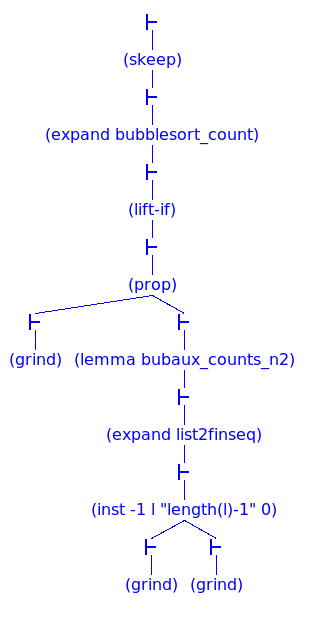
\includegraphics[width=\linewidth,trim={0 0 0 0},clip]{figures/bubblesort-count.png}
    \caption{A prova do lema de complexidade do \texttt{bubblesort\_count}
    é direta a partir da aplicação do lema \ref{lemma:bacount}, pois sabemos
    os valores exatos de $n$ e $c$, para uma dada lista $l$, que serão passados
    para \texttt{bubblesort\_aux}.}
    \label{fig:bsort1}
\end{minipage}
\hfill
\begin{minipage}{0.475\linewidth}
    \centering
    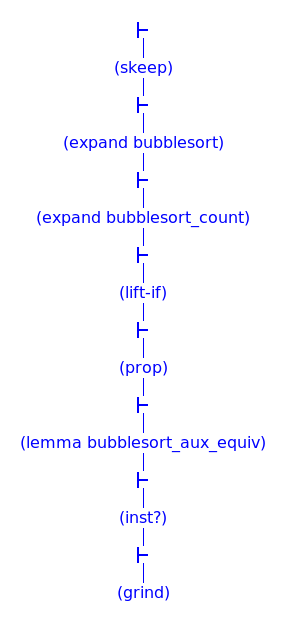
\includegraphics[width=\linewidth,
    trim={0 0 0 0},clip]{figures/bubblesort-equiv.png}
    \caption{A prova de equivalência entre \texttt{bubblesort} e
    \texttt{bubblesort\_count} é direta a partir da aplicação do
    lema \ref{lemma:baequiv}.}
    \label{fig:bsort2}
\end{minipage}
\end{figure}

\subsection{TCCs}

Ao final das provas dos lemas elaborados ainda restaram alguns TCCs 
(\textit{Type-Correctness Conditions}) que não puderam ser verificados
automaticamente pelo PVS. Isto foi parcialmente resolvido após uma mudança
na ordem em que os lemas foram enunciados no arquivo de entrada.
Faltou, contudo, realizar a prova de TCCs relacionados com a função
\texttt{bubbling}, e estes precisaram ser provados manualmente, pois necessitaram
de uma prova um pouco mais elaborada, embora ainda relativamente curta. A título
de exemplo, apresentaremos o \texttt{bubbling\_TCC3}, mas os
outros consistiam de sequentes semelhantes relacionados ao comprimento
de partes das listas.
\begin{lstlisting}
  |-------
{1}   FORALL (l: list[nat], (n: below[list2finseq[nat](l)`length])):
        car(l) > car(cdr(l)) AND NOT n = 0 IMPLIES
         n - 1 >= 0 AND n - 1 < list2finseq[nat]
               (cons[nat](car[nat](l), cdr[nat](cdr[nat](l))))`length
\end{lstlisting}

A prova deste sequente foi direta e se deu principalmente pela expansão
de \texttt{list2finseq}, e posteriormente a manipulação das definições
de \texttt{length} que surgiram (Figura \ref{fig:tcc}).


\begin{figure}[H]
\begin{minipage}{0.45\linewidth}
    \centering
    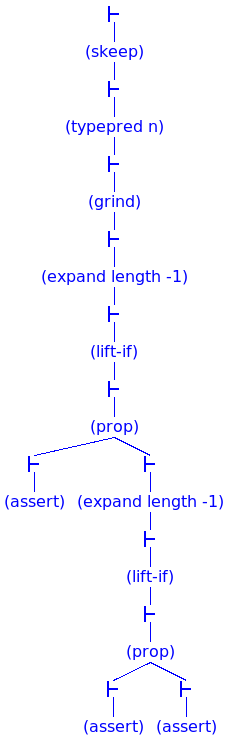
\includegraphics[height=0.4\textheight,width=0.8\linewidth,trim={0 9.7cm 0 0},clip]{figures/bubbling-tcc3.png}
\end{minipage}
\hfill
\begin{minipage}{0.45\linewidth}
    \centering
    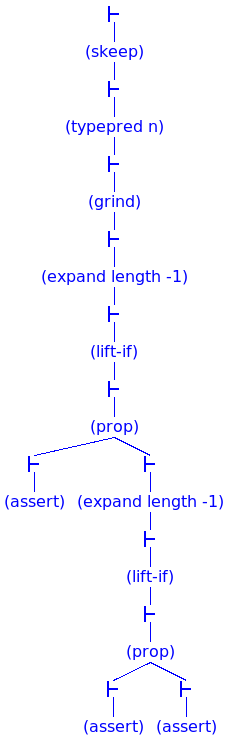
\includegraphics[height=0.4\textheight,width=0.8\linewidth,
    trim={0 0 0 9.7cm},clip]{figures/bubbling-tcc3.png}
\end{minipage}
    \caption{Prova do TCC \texttt{bubbling\_TCC3} que não pode ser completado
    automaticamente pelo PVS.}
    \label{fig:tcc}
\end{figure}

